\newpage
\section*{Design of the system (Problem 5, 6)\footnote{Problem 5 and 6 were combined as explaining the thruster configuration and the single line diagram independently lead to repeating a lot of the same arguments}} \label{prob_5and6}

\todo[inline]{Things that \textbf{have to} be answered \\     \begin{itemize}
    \item Include the diagram for the propulsion system/segregations 
    \item Disuse the segregations for the power \textbf{and} the thruster system
        \subitem{Thrusters}
        \subitem{Feeders cables}
        \subitem{Gensets}
        \subitem{Machine rooms}
        \subitem{Sectioning of main switchboard}
        \subitem{Requirements for the bus-tie breakers}
    \item Include our SLD
    \item Explain the worst-case failure based on our SLD
    \item Explain how our design still provides the required propulsion power
\end{itemize}}

 \subsubsection*{The design philosophy}\label{Sec:designPhilosophy}
The philosophy when designing the power system and the thruster configuration was most off all to make a system that is realistic, in accordance to the applicable standards and the industry uses \todo{Rewrite, not sure what you mean here. -H}. If a DP system fail it can lead to hazards and serious consequences. Therefore, effort was putt into making the system more reliable than the minimum requirements and this includes multiple levels of redundancy. In order to make the system as realistic as possible, it was also decided to try to make sure the equipment that was used in the project was available in the market today. Also, the load level on the generators were considered in order to make them work within a reasonable load level. However, it was not necessary to do that with the thrusters, since its power demand was given, thus out of the scope of the project. 


\subsubsection*{Industry Practices} \label{Sec:industryPractices}
Based on the single-line diagrams and thruster configurations of semi-submersibles used today, it can be seen that the most common arrangement is to use four redundancy groups for the generation and one to two thrusters placed in each corner of the pontoons. These kind of configurations can be seen in the example configuration from the lecture notes and the diagram for the semi-sub "DEEPWATER HORIZON" found in Appendix \ref{Sec:ThrusterConfiguratons}.  

\subsection*{Design requirements} \label{Sec:designRequirements}
As summary of the requirements given in the problem description is summed up in Table \ref{tab:designRequirements}. It was assumed that the service load during worst-case failure stayed the same at 4MW, the same as during single failure. The service loads under normal operation was assumed to be three times that of the single failure load, so totally 12MW.  

\begin{table}[h]
    \centering
    \begin{tabular}{l c c}
                        & \text{Normal Operation [MW]} & \text{Worst-case Failure [MW]}  \\
    \toprule
    \text{Propulsion Power}     & 42                   &  34  \\
    \text{Service Loads}        & 12                   &  4  \\
    \text{Drilling Power}       & 12                   &  0  \\
    \midrule
    \text{Total Loads}          & 66                   &  38 \\
    \bottomrule
    \end{tabular}
    \caption{Design requirements}
    \label{tab:designRequirements}
\end{table}



\subsection*{The System Design}\todo[inline]{\begin{itemize}
    \item Needs a better title
    \item We changed the cabling so that the propulsion- and drilling efficiency changed compared to the numbers here. The numbers will have to be updated
\end{itemize}}

\subsubsection*{Definition of worst-case failure} \label{Sec:worstCaseFailure}
DNV GL definition of worst case failure is explained in Section \nameref{Sec:3d}. In short, it states that DNV GL defines the worst-case failure as the (single) failure that causes the loss of the most significant redundancy group. In this case, that would correspond to loosing one redundancy group. However, there might be worse scenarios, and since a failure of a DP system on a rig would have potentially significant consequences. Therefore, to lower the risk levels (environmental, to human life or financial), it is desirable that the system is more redundant than the minimum requirement. In order to ensure that, the rig was designed such that it would also be able to hold its position if two redundancy groups were out of service. This was defined as this rig's worst case failure condition and is that is mean when the term \textit{worst-case failure} is used for the rest of the report. %\todo[inline]{Add why an incident such as flooding would cause two compartments to be lost and explain that this needs to be taken into account since the rig should be classed as DYNPOS(AUTRO)\cite{RulesShipsDNVGLPart6Chap3}.}
 
% Previous sentence about risk: both to avoid potential environmental damage, large costs etc. Therefore 
 
\subsubsection*{Location of the thrusters}
Under normal DP operation, it is common practice to have at least one thruster in each corner in operation \cite{RedundantDesignIntention_DNV}.
This improves the rig's maneuverability, therefore its capability of hold itself in place. A standard redundancy measure would therefore be to have at least two thrusters in each corner. This is consistent with what is normal industry practice as described before. This configuration can for example be seen used for the "DEEPWATER HORIZON" which can be found in Appendix \ref{Sec:ThrusterConfiguratons}. 
 
\begin{minipage}{.5\textwidth}
  TEXT 1
\end{minipage}
\noindent\begin{minipage}{.5\textwidth}
  \begin{figure}
    %\centering
    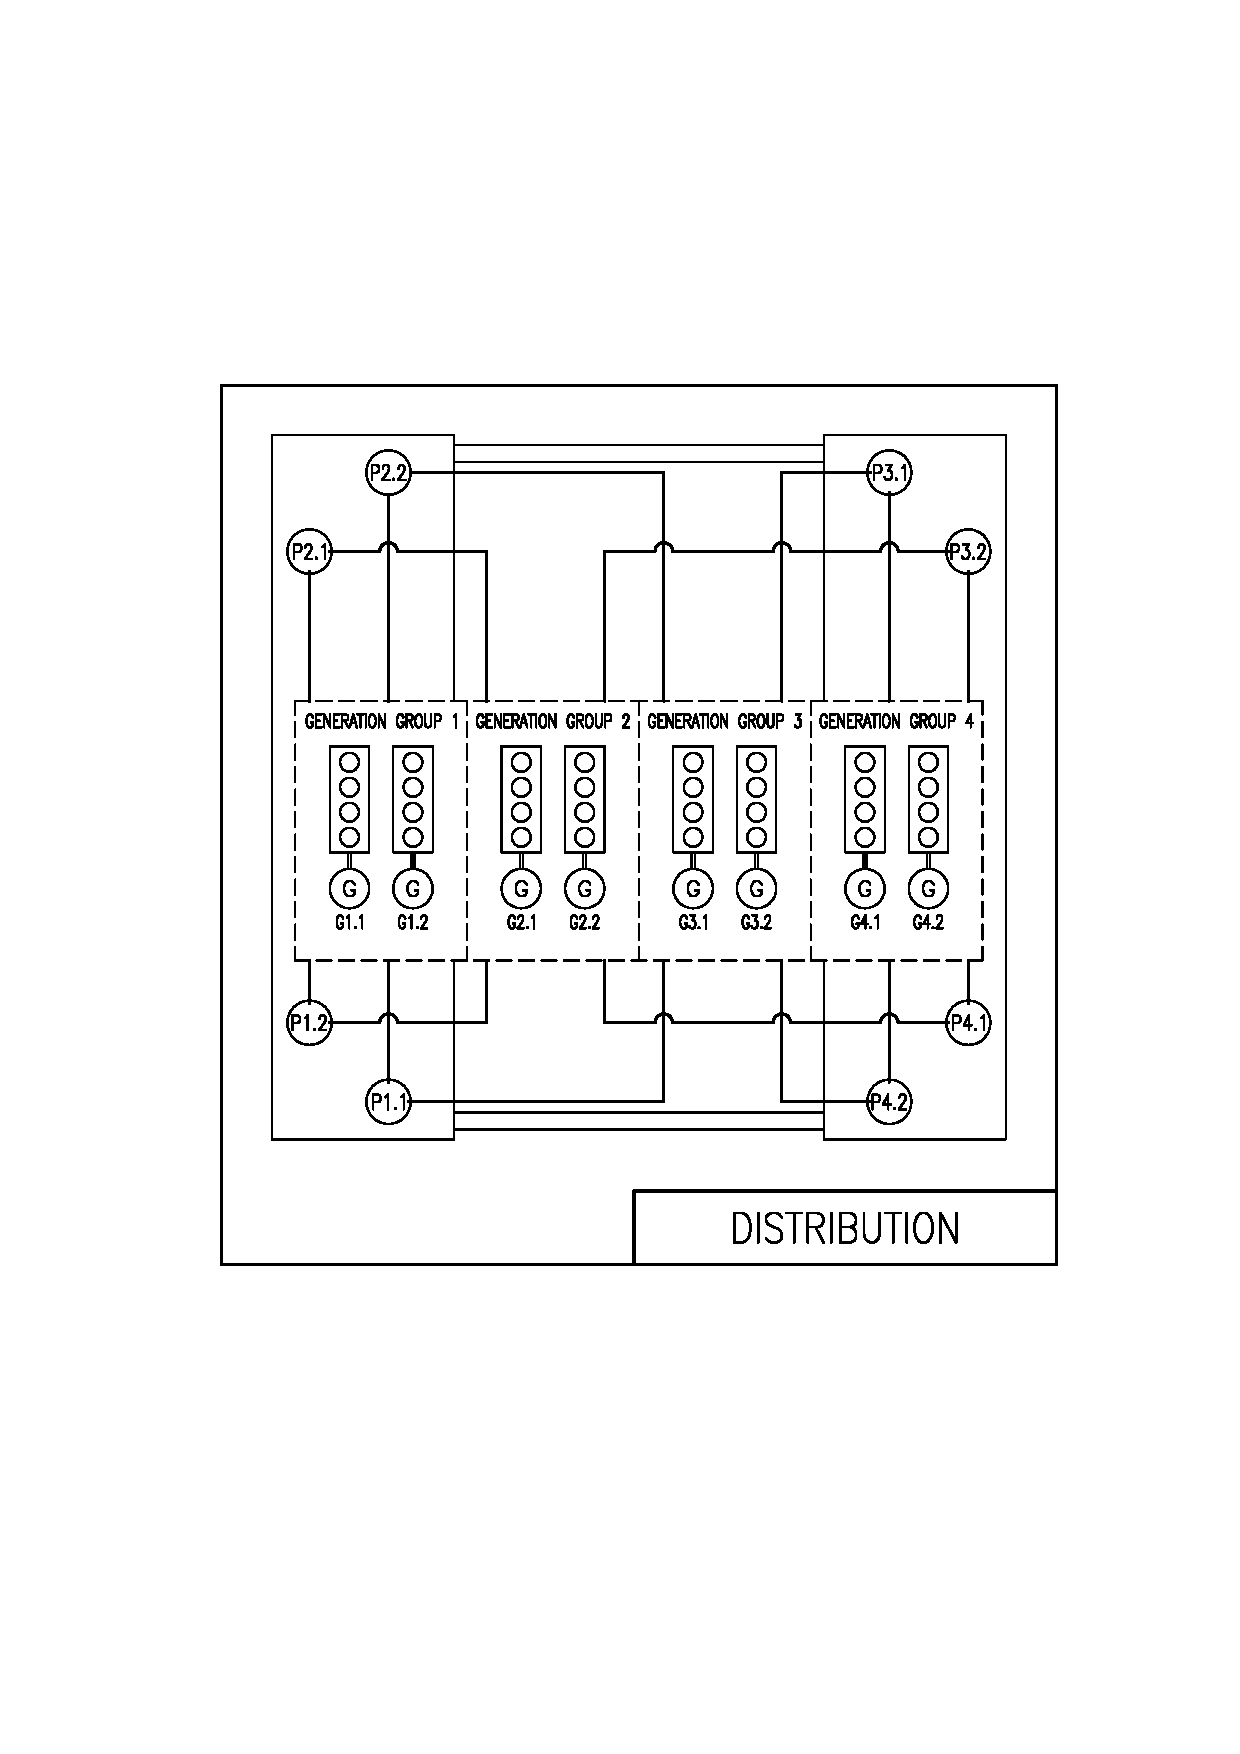
\includegraphics[]{figures/Single_Line_distribution.pdf}
    \caption{Thruster configuration}
    \label{fig:SingleLineDiagram}
\end{figure}
\end{minipage}

 

\begin{table}[H]
    \centering
    \begin{tabular}{l|cc|cc|cc|cc}
    \text{Propulsion units:} & 1.1 & 1.2 & 2.1 & 2.2 & 3.1 & 3.2 & 4.1 & 4.2 \\
    \hline
    %\toprule
    \text{Generation group 1} & X & X & X & X &   &   &   &    \\
    \text{Generation group 2} &   & X & X &   &   & X & X &    \\
    \text{Generation group 3} & X &   &   & X & X &   &   & X\\
    \text{Generation group 4} &   &   &   &   & X & X & X & X  \\
    \end{tabular}
    \caption{Generation-group-to-propulsion-units connections}
    \label{tab:genGroupToThruster}
\end{table}


 
 
 
 \section*{New Section}
\begin{table}[h!]
    \centering
    \begin{tabular}{l l}
        \text{Component} & \text{Efficiency} \\
        \toprule
        \text{Switchboard ($\eta_s$)}         & $\eta_s$ = 0.999  \\
        \text{3-Phase Transformer ($\eta_t$)} & $\eta_t$ = 0.993  \\
        \text{Frequency Converter ($\eta_f$)} & $\eta_f$ = 0.985  \\
        \text{Electric Motor ($\eta_m$)}      & $\eta_m$ = 0.960  \\
    \bottomrule
    \end{tabular}
    \caption{Efficiency individual components}
    \label{tab:efficiencies}
\end{table}

\begin{table}[H]
    \centering
    \begin{tabular}{l r r r}
    & \text{Efficiency calculation [-]} & \text{Normal Operation [MW]} & \text{Worst-case Failure [MW]}  \\
    \toprule
    \rule{0pt}{12pt}\text{Propulsion}     & $\eta_p  = \eta_s^2\cdot\eta_t\cdot\eta_f\cdot\eta_m  = 0.937$ & $\frac{1}{\eta_p}\cdot$42  = 44.84  & $\frac{1}{\eta_p}\cdot$34 = 36.30   \\
    \rule{0pt}{12pt}\text{Service load}        & $\eta_{sl} = \eta_s  = 0.999$     & $\frac{1}{\eta_{sl}}\cdot$12 = 13.01  & $\frac{1}{\eta_{sl}}\cdot4$ =  4.00 \\
    \rule{0pt}{12pt}\text{Drilling}       & $\eta_d  = \eta_s^2 \cdot\eta_t\cdot\eta_f^2\cdot\eta_m = 0.923$   & $\frac{1}{\eta_d}\cdot$12 = 13.00  & 0   \\
    \midrule
    \text{Total}          &     & 69.86  & 40.30  \\
    \bottomrule
    \end{tabular}
    \caption{Power demand from the generators}
    \label{tab:powerDemand}
\end{table}

\begin{table}[H]
    \centering
    \begin{tabular}{l l l l l l l}
        \text{Number of gensets in service} & 3 & 4 & 5 & 6 & 7 & 8 \\
        \toprule
        \text{Normal Operation (66MW)}   & - & - & - & 83.16\% & 71.29\% & 62.37\% \\
        \text{Worst-case failure (38MW)}  & 95.96\% & 71.97\% & 57.58\%\footnote{Only 1 failed compartment} &  47.98\%\footnote{Only 1 failed compartment} & - & - \\
        \bottomrule
    \end{tabular}
    \caption{Load on 14MW gensets}
    \label{tab:gensetLoad}
\end{table}

